\documentclass[../zavrsni.tex]{subfiles}

\begin{document}

\sloppy

\justifying

\section{Sustavi za rad u stvarnom vremenu}

Sustavi za rad u stvarnom vremenu (engl. \textit{real-time system}) danas su neizostavan dio mnogih sustava korištenih u svim
granama ljudske djelatnosti. Kod njih nije bitan samo rezultat izvođenja operacije, nego je jednako važno 
i vrijeme u kojem se ta operacija izvede. Zbog toga se svakom zadatku pridjeljuje krajnji rok do kojeg se mora izvršiti. 
Kako bi sustav radio pouzdano, mora se osigurati predvidivo raspoređivanje zadataka koje će osigurati da se što više 
zadataka izvrši na vrijeme.
SRSV mora imati implementiranu kontrolu zadataka, kontrolu vremena, raspoređivač zadataka i sustav komunikacije i sinkronizacije
među zadatcima.

S obzirom na posljedice koje izaziva propuštanje roka izvršavanja zadatke dijelimo u četiri skupine :
\begin{itemize}
    \item[--] strogi zadatci (engl. \textit{hard real-time tasks}),
    \item[--] ublaženi zadatci (engl. \textit{soft real-time tasks}),
    \item[--] čvrsti zadatci (engl. \textit{firm real-time tasks}),
    \item[--] opcionalni zadatci (engl. \textit{non real-time tasks}).
\end{itemize}

\begin{figure}[!htb]
  \center{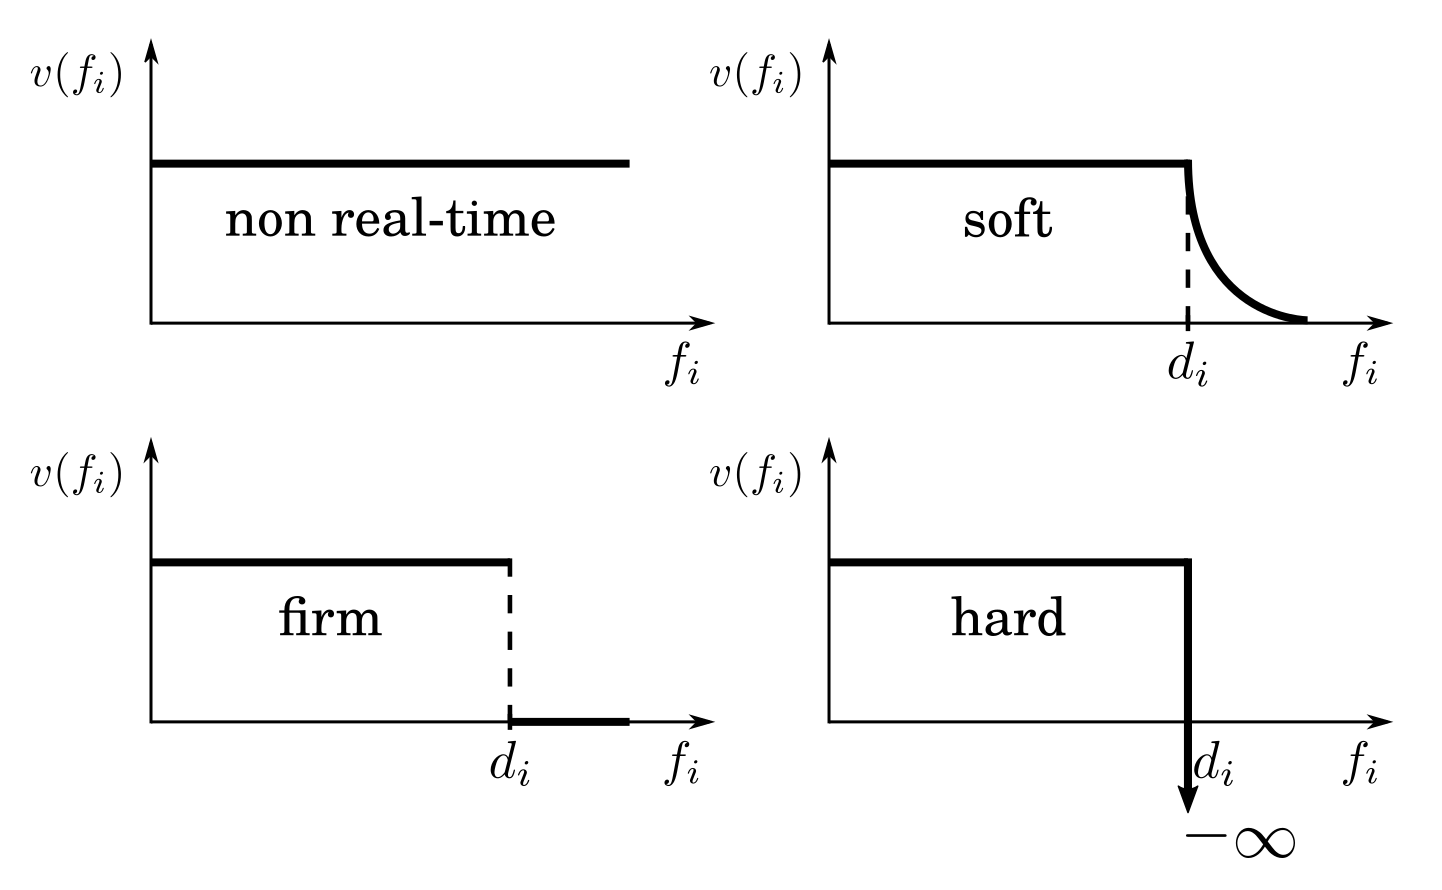
\includegraphics[width=\textwidth]
  {images/4_vrste.png}}
  \caption{\label{fig:my-label} 4 vrste zadataka u SRSV-u}
\end{figure}

Strogi zadatci niti jednom ne smiju propustiti krajnji rok izvršavanja jer su to zadatci koji obavljaju važan posao. Njihovo 
propuštanje izaziva katastrofalne posljedice koje mogu biti pogubne za cijeli sustav i njegovu okolinu. Dobar primjer strogog zadatka je detekcija 
pritiska papučice kočnice na automobilu. Taj zadatak je kritičan i propuštanje njegovog izvršenja za posljedicu može imati ozbiljnu
nesreću s ljudskim žrtvama. Čvrsti zadatci su oni čije prekasno izvršavanje ne donosi korist sustavu, ali mu ni ne šteti.
Za razliku od čvrstih, kod ublaženih zadataka čak i izvršavanje poslije krajnjeg roka izvršavanja donosi korist sustavu.
Primjer ovakvog zadatka je paljenje signalne lampice ili prikaz podataka na pokazniku.
Na kraju, imamo zadatke koji su opcionalni i nisu vremenski ograničeni, te donose jednaku korist sustavu kad god se izveli.
Na slici 2.1 prikazana je ovisnost koristi koju izvršavanje posla donosi sustavu o vremenu izvršavanja posla za sva 4 opisana slučaja.

Zadatci u operacijskim sustavima za rad u stvarnom vremenu općenito se mogu naći u jednom od 3 stanja, a to su:
\begin{itemize}
    \item[--] zadatak koji se trenutno izvodi (engl. \textit{running task}),
    \item[--] zadatci koji su spremi za izvođenje (engl. \textit{ready tasks}),
    \item[--] zadatci koji su blokirani i čekaju određeni događaj (engl. \textit{blocked tasks}).
\end{itemize}

Kod sustava s jednom procesorskom jezgrom, u određenom trenutku može se izvoditi samo jedan zadatak.
Zadatci koji su spremni za izvođenje
čekaju oslobođenje procesora i jedan od njih se odabire za izvršavanje.
Dio jezgre SRSV-a koji je zadužen za izbor zadatka koji je spreman za izvođenje i koji će se idući izvršavati naziva se raspoređivač 
zadataka (engl. \textit{task scheduler}). To je najvažniji dio jezgre SRSV-a jer o raspoređivanju zadataka ovisi kolika će biti kvaliteta usluge i
koliko pouzdan će biti cijeli sustav.
Neki zadatci mogu biti privremeno ili trajno blokirani i dok su u tom stanju raspoređivač zadataka ih ne uzima u obzir.
Zadatci se tijekom rada prebacuju između opisanih stanja, no treba napomenuti da je ovo generalna podjela koja se razlikuje u 
implementaciji konkretnih SRSV-ova.

\begin{figure}[!htb]
    \center{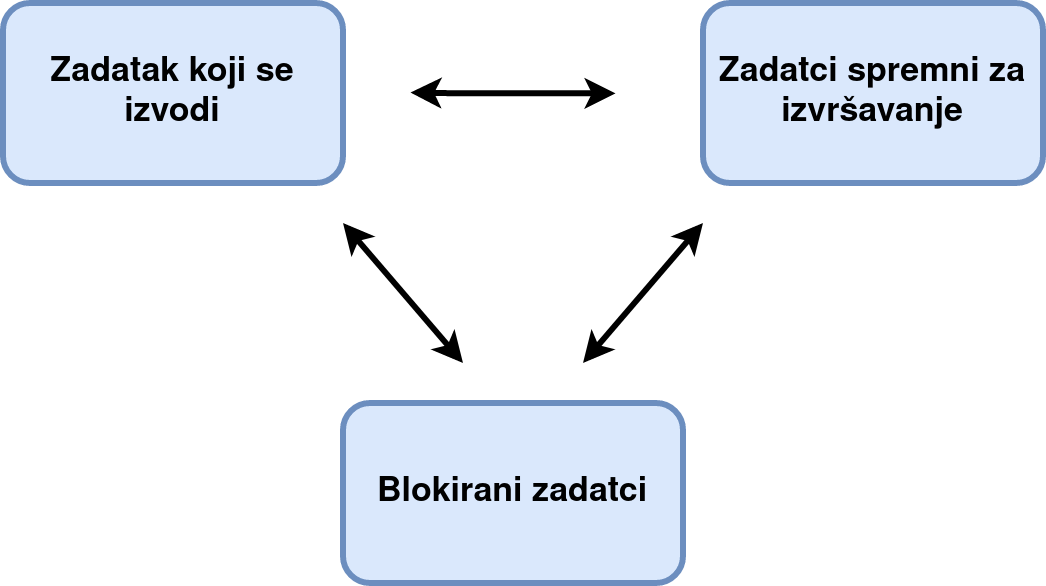
\includegraphics[width=\textwidth]
    {images/stanja_taskova.png}}
    \caption{\label{fig:my-label} Stanja zadataka u SRSV-u}
  \end{figure}

\section{Periodični zadatci u sustavima za rad u stvarnom \\vremenu}

Općenito, zadatci u sustavima za rad u stvarnom vremenu se označavaju sa $\tau_i$, gdje je $i$ identifikator pojedinog zadatka. 
Periodični zadatci su zadatci koji se iznova ponavljaju u istim vremenskim intervalima $T_i$. Taj interval naziva se period zadatka.
Dio zadatka izvršen u jednom periodu naziva se posao.
Drugi parametar koji opisuje zadatak je trajanje njegova izvršavanja $C_i$ (engl. \textit{computation time}). Period i vrijeme izvršavanja zajedno daju veličinu 
koju nazivamo faktor opterećenja (engl. \textit{utilization factor}):
\begin{equation*}
  U\textsubscript{i} = \frac{C\textsubscript{i}}{T\textsubscript{i}}
\end{equation*}
Ova veličina daje postotak zauzeća procesora zadatkom $\tau_i$ u jednom periodu $T_i$. S obzirom na to da se poslovi
ponavljaju jedan za drugim, to je ujedno i veličina koja govori koliko procesorskog vremena se ukupno troši na zadatak $\tau_i$.

Nadalje, bitna veličina koja opisuje svaki zadatak je krajnji rok njegova završetka (engl. \textit{deadline}). Krajnji rok izvršavanja je vrijeme 
do kojeg se posao mora izvršiti kako bi donio korist sustavu. U ovom radu razmatrani su 
isključivo zadatci čiji je krajnji rok završetka jednak periodu. Takav krajnji rok naziva se implicitni krajnji rok završetka. 
Kao primjer dan je vremenski dijagram s jednim periodičnim zadatkom.
Period zadatka iznosi 4 vremenske jedinice, a vrijeme izvršavanja pojedinog posla 1 vremensku jedinicu. Pomoću ta dva podatka i ranije 
dane formule proizlazi da je faktor opterećenja zadatka 0.25. Drugim riječima, ovaj zadatak zauzima 25 \% ukupnog procesorskog vremena.

\begin{figure}[h]
    \centering

    \begin{RTGrid}[width=13cm]{1}{8}

      \TaskArrDead{1}{0}{4}     
      \TaskArrDead{1}{4}{4}
    %  \TaskArrDead{1}{8}{4}
     % \TaskArrDead{1}{12}{4}
     % \TaskArrDead{1}{16}{4}
      \TaskArrival{1}{8}
  
      \TaskExecution{1}{0}{1}
      \TaskExecution{1}{4}{5}
     % \TaskExecution{1}{8}{9}
     % \TaskExecution{1}{12}{13}
     % \TaskExecution{1}{16}{17}

    \end{RTGrid}

    \caption{Primjer periodičnog zadatka}
    \label{fig:ex1}
  \end{figure}

Ukupno opterećenje sustava dobiva se kao zbroj faktora opterećenja svih zadataka. 
\begin{equation*}
    U = \sum_{i=1}^{N}\frac{C\textsubscript{i}}{T\textsubscript{i}}
\end{equation*}
Ako je sustav preopterećen, tj. ukupno opterećenje mu 
je veće od 1, neki od zadataka se neće izvršiti do svog roka za izvršavanje. U tom slučaju koriste se algoritmi koji će osigurati 
da se zadatci ne preskaču nasumično, već na kontroliran način kao bi se sustav zaštitio od potencijalnih oštećenja nastalih preskakanjem 
kritičnih zadataka. Postoje dvije vrste preopterećenja sustava.
\begin{itemize}
    \item[--] trajno preopterećenje (engl. \textit{permanent overload}),
    \item[--] prolazno preopterećenje (engl. \textit{transient overload}).
\end{itemize}
Kod prolaznog opterećenja sustav ima ukupno opterećenje manje ili jednako 1, no u nekom trenutku može doći do aktivacije aperiodičnog zadatka 
koji onda sustav gura u stanje preopterećenja. Nakon što prođe određeno vrijeme i aperiodični zadatak se izvede, sustav se vraća u prijašnje
stanje i svi zadatci se izvršavaju pravovremeno. Drugi slučaj je kada je sustav u stanju trajnog preopterećenja, kada je ukupno 
opterećenje sustava trajno veće od 1. Tada se svi poslovi neće moći izvršiti i kontinuirano će se pojedini poslovi morati propuštati. 

%treba li dodati vrste weakly hard uvjeta

U ovom radu ispitivat će se ponašanje sustava s ublaženo-strogim uvjetima (engl. \textit{weakly-hard constraints}). Za razliku od 
strogih zadataka, kod ublaženo-kritičnih zadataka povremeno dopuštamo da se zadatak ne izvede na vrijeme, ali na predvidiv i 
kontroliran način. U određenom vremenskom okviru točno se određuju pravila propuštanja zadataka. Postoje 4 modela SRSV-a s ublaženo-strogim uvjetima :
\begin{itemize}
    \item[--] u $m$ slijednih perioda posao se mora pravovremeno izvršiti u njih $n$,
    \item[--] u $m$ slijednih perioda posao se mora pravovremeno izvršiti u njih $n$ koji slijede jedan za drugim,
    \item[--] u $m$ slijednih perioda posao se ne smije propustiti više od $n$ puta,
    \item[--] u $m$ slijednih perioda posao se ne smije propustiti u njih $n$ koji slijede jedan za drugim.
\end{itemize}

\section{Skip-over model zadataka ublaženo-strogih uvjeta}

U ovom radu istražen je model u kojem se u $S_i$ slijednih perioda zadatak $\tau_i$ ne smije propustiti više od jednom (engl. \textit{skip-over model}).
Broj $S_i$ naziva se faktor propuštanja (engl. \textit{skip-over factor}).
Prema tom modelu 
poslovi se dijele na one koji se moraju izvršiti (crveni poslovi) i na one čije je izvršavanje opcionalno (plavi poslovi). Posao se proglašava crvenim 
ako je jedan od prošlih $S_i-1$ poslova nije pravovremeno izvršio.
Na temelju važnosti pojedinog zadatka za rad cjelokupnog sustava određuje se u koliko slijednih perioda 
se zadatak može jednom propustiti. Ovaj pristup osigurava znatno bolje ponašanje u uvjetima preopterećenja jer se propuštanje
pojedinih poslova odvija deterministički.

Opisani model jednostavno možemo opisati pomoću njegove dvije karakteristike:
\begin{itemize}
  \item[--] ako se plavi posao ne izvede na vrijeme, sljedećih $S_i-1$ poslova se proglašava crvenima,
  \item[--] ako se plavi posao izvede do svog krajnjeg roka za izvršavanje, sljedeći posao je također plavi.
\end{itemize}

Dvije posebne vrijednosti faktora propuštanja su 1 i $\infty$. $S_i=1$ govori da su svi poslovi zadatka $\tau_i$ uvijek plavi i uvijek se 
mogu propustiti. S druge strane $S_i=\infty$ označava da su svi poslovi crveni i da se niti jedan ne smije propustiti.

\section{Algoritmi za raspoređivanje zadataka}

U ovom radu ispitivat će se različiti algoritmi za raspoređivanje zadataka u sustavu koji se nalazi u stanju trajnog preopterećenja.
U navedenom slučaju važno je osigurati preskakanje zadataka na predvidiv i za sustav siguran način.

Mjera kojom će se uspoređivati učinkovitost pojedinih algoritama naziva se kvaliteta usluge (engl. \textit{quality of service}).
Računa se kao omjer broj zadataka koji su se izvršili do krajnjeg roka završetka i ukupnog broja svih zadataka.

% popravi da š bude u formuli
\begin{equation*}
    QoS = \frac{\text{broj izvršenih poslova do krajnjeg roka}}{\text{ukupan broj poslova}}
\end{equation*}

U nastavku su opisani korišteni algoritmi za raspoređivanje zadataka.
Za svaki algoritam dan je primjer generiranog rasporeda na jednostavnom skupu zadataka koji je dan u tablici 2.1. 
Raspored se prikazuje vremenskim dijagramom u kojem
je vidljivo koji zadatak se u danom trenutku izvršava. 
Za dani set zadataka zadano je da je prvi
zadatak kritičan i mora se uvijek izvršiti, drugi zadatak ne utječe na sigurnost sustava, a treći zadatak mora se izvršiti svaki drugi put.

\begin{table}[h!]
    \begin{center}
      \begin{tabular}{||c || c | c | c | c||} 
       \hline
       Zadatak & Period & Vrijeme izvršavanja & Faktor propuštanja & Faktor opterećenja \\ [0.5ex] 
       \hline\hline
       $\tau_1$ & 6 & 2 & $\infty$ & 0.33 \\ 
       \hline
       $\tau_2$ & 8 & 2 & 1 & 0.25 \\
       \hline
       $\tau_3$ & 4 & 2 & 2 & 0.50 \\
       \hline
      \end{tabular}
    \end{center}
    \caption{\label{tab:table-name}Skup zadataka korišten u primjerima}
    \end{table}

Dani set zadataka nalazi se u preopterećenju, i neki od zadataka neće zadovoljiti svoj krajnji rok završetka. Ukupni faktor opterećenja
sustava je 1.08.

\subsection{Algoritam EDF}

Algoritam EDF (engl. \textit{earliest deadline first}) je algoritam koji pri raspoređivanju zadataka najveći prioritet daje onim poslovima 
koji imaju najbliži krajnji rok završetka. 
Ako sustav nije preopterećen (ako je ukupni faktor opterećenja manji ili jednak 1) 
ovim algoritmom optimalno će se rasporediti zadatci i svi će se izvršiti. Ovaj algoritam nije pogodan za primjenu s ublaženo strogim uvjetima 
jer ne pruža mehanizam koji garantira zadovoljenje ublaženo-strogih uvjeta,  
ali u ovom radu je istražen jer se u praksi često koristi. 
Raspored generiran algoritmom EDF prikazan je na slici 2.4.
Na vremenskom dijagramu crnom bojom su prikazani poslovi koji su propustili svoj krajnji rok izvršenja.

\begin{figure}[h!]
    \centering

    \begin{RTGrid}[width=13cm]{3}{24}

      \TaskArrDead{1}{0}{6}     
      \TaskArrDead{1}{6}{6}
      \TaskArrDead{1}{12}{6}
      \TaskArrDead{1}{18}{6}
      \TaskArrival{1}{24}
  
      \TaskExecution{1}{2}{4}
      \TaskExecution{1}{9}{11}
      \TaskExecution{1}{16}{18}
      \TaskExecution[color=black]{1}{23}{24}

      \TaskArrDead{2}{0}{8}     
      \TaskArrDead{2}{8}{8}
      \TaskArrDead{2}{16}{8}
      \TaskArrival{2}{24}
  
      \TaskExecution{2}{4}{7}
      \TaskExecution{2}{13}{16}
      \TaskExecution{2}{20}{23}

      \TaskArrDead{3}{0}{4}     
      \TaskArrDead{3}{4}{4}
      \TaskArrDead{3}{8}{4}
      \TaskArrDead{3}{12}{4}
      \TaskArrDead{3}{16}{4}
      \TaskArrDead{3}{20}{4}
      \TaskArrival{3}{24}
  
      \TaskExecution{3}{0}{2}
      \TaskExecution[color=black]{3}{7}{9}
      \TaskExecution[color=black]{3}{11}{13}
      \TaskExecution{3}{18}{20}

    \end{RTGrid}

    \caption{Raspored zadataka algoritmom EDF}
    \label{fig:ex1}
  \end{figure}

\subsection{Algoritam RTO}

Algoritam RTO (engl. \textit{red tasks only}) je prvi i najjednostavniji algoritam korišten za skip-over model SRSV-a s ublaženo-strogim uvjetima.
U njemu je implementiran mehanizam za uvažavanje faktora propuštanja $S_i$ kod raspoređivanja zadataka.
Prema algoritmu RTO samo se izvršavaju crveni poslovi, dok se oni koji se mogu preskočiti uvijek preskaču. 
Time je osigurano poštivanje zadanih uvjeta, no pri manjim 
faktorima opterećenja ovaj algoritam nije optimalan. Razlog tomu je to što postoji slobodno procesorsko vrijeme u kojem bi se mogli 
izvršiti zadatci koje nije nužno izvršiti, no oni se automatski izbacuju iz rasporeda. Strogi zadatci raspoređuju se prema 
ranije opisanom algoritmu EDF. Raspored generiran algoritmom BWP prikazan je na slici 2.5. 

\begin{figure}[h!]
    \centering

    \begin{RTGrid}[width=13cm]{3}{24}

        \TaskArrDead{1}{0}{6}     
        \TaskArrDead{1}{6}{6}
        \TaskArrDead{1}{12}{6}
        \TaskArrDead{1}{18}{6}
        \TaskArrival{1}{24}
    
        \TaskExecution[color=red]{1}{0}{2}
        \TaskExecution[color=red]{1}{6}{8}
        \TaskExecution[color=red]{1}{12}{14}
        \TaskExecution[color=red]{1}{18}{20}
  
        \TaskArrDead{2}{0}{8}     
        \TaskArrDead{2}{8}{8}
        \TaskArrDead{2}{16}{8}
        \TaskArrival{2}{24}
    
        \TaskArrDead{3}{0}{4}     
        \TaskArrDead{3}{4}{4}
        \TaskArrDead{3}{8}{4}
        \TaskArrDead{3}{12}{4}
        \TaskArrDead{3}{16}{4}
        \TaskArrDead{3}{20}{4}
        \TaskArrival{3}{24}
    
        \TaskExecution[color=red]{3}{2}{4}
        \TaskExecution[color=red]{3}{8}{10}
        \TaskExecution[color=red]{3}{16}{18}

    \end{RTGrid}

    \caption{Raspored zadataka algoritmom RTO}
    \label{fig:ex1}
  \end{figure}


\subsection{Algoritam BWP}

Algoritam BWP (engl. \textit{blue when possible}) je poboljšanje ranije opisanog RTO algoritma. Kod BWP algoritma prioritet imaju strogi zadatci, 
no raspoređuju se i zadatci koji se ne moraju nužno izvesti. Na taj način, ako se svi strogi zadatci izvrše, na red će doći
i opcionalni zadatci. Ovom modifikacijom znatno se poboljša kvaliteta usluge, pogotovo pri
 manjim faktorima opterećenja. Zadatci su u dijagramu obojeni prema nazivu algoritma, crvena boja za stroge zadatke, a plava za zadatke 
 čije izvršavanje je opcionalno. Raspored generiran algoritmom BWP prikazan je na slici 2.6.

 \begin{figure}[h!]
    \centering

    \begin{RTGrid}[width=13cm]{3}{24}

        \TaskArrDead{1}{0}{6}     
        \TaskArrDead{1}{6}{6}
        \TaskArrDead{1}{12}{6}
        \TaskArrDead{1}{18}{6}
        \TaskArrival{1}{24}
    
        \TaskExecution[color=red]{1}{0}{2}
        \TaskExecution[color=red]{1}{6}{8}
        \TaskExecution[color=red]{1}{12}{14}
        \TaskExecution[color=red]{1}{18}{20}
  
        \TaskArrDead{2}{0}{8}     
        \TaskArrDead{2}{8}{8}
        \TaskArrDead{2}{16}{8}
        \TaskArrival{2}{24}
    
        \TaskExecution[color=blue]{2}{10}{12}
        \TaskExecution[color=blue]{2}{20}{22}
  
        \TaskArrDead{3}{0}{4}     
        \TaskArrDead{3}{4}{4}
        \TaskArrDead{3}{8}{4}
        \TaskArrDead{3}{12}{4}
        \TaskArrDead{3}{16}{4}
        \TaskArrDead{3}{20}{4}
        \TaskArrival{3}{24}
    
        \TaskExecution[color=red]{3}{2}{4}
        \TaskExecution[color=blue]{3}{4}{6}
        \TaskExecution[color=red]{3}{8}{10}
        \TaskExecution[color=blue]{3}{14}{16}
        \TaskExecution[color=red]{3}{16}{18}
        \TaskExecution[color=blue]{3}{22}{24}

    \end{RTGrid}

    \caption{Raspored zadataka algoritmom BWP}
    \label{fig:ex1}
  \end{figure}

\subsection{Usporedba opisanih algoritama}

U tablici 2.2 prikazana je usporedba ranije opisanih algoritama na primjeru danom u tablici 2.1. Za svaki algoritam prikazana je 
kvaliteta usluge i broj kršenja postavljenih ublaženo-strogih uvjeta. 
Vidljivo je kako su kod algoritama RTO i BWP zadovoljeni svi uvjeti postavljeni nad simulacijom, uz razliku što algoritam BWP daje 
znatno veću kvalitetu usluge. Algoritam EDF ne osigurava poštivanje zadanih ublaženo-strogih uvjeta te time nije pogodan za kontrolne 
aplikacije s kritičnim poslovima u stanju preopterećenja.

\begin{table}[h!]
  \begin{center}
    \begin{tabular}{||c || c | c ||} 
     \hline
     Algoritam & Kvaliteta usluge & Broj kršenja ublaženo-strogih uvjeta \\ [0.5ex] 
     \hline\hline
     EDF & 0.62 & 3 \\ 
     \hline
     RTO & 0.54 & 0 \\
     \hline
     BWP & 0.92 & 0 \\
     \hline
    \end{tabular}
  \end{center}
  \caption{\label{tab:table-name}Usporedba opisanih algoritama}
  \end{table}

\end{document}